\documentclass[12pt]{article}
\usepackage{amsmath}
\usepackage{amssymb}
\usepackage{amsthm}
\usepackage{accents}
\usepackage{graphicx}
\usepackage{amsfonts}
\setlength{\oddsidemargin}{0in}
\setlength{\textwidth}{6.5in}
\setlength{\topmargin}{-.55in}
\setlength{\textheight}{9in}
\pagestyle{empty}
\renewcommand \d{\displaystyle}
\begin{document}
\noindent Dallas Klumpe

\noindent Math 4310

\noindent HW 8\\
\noindent Section 34\\

2.a. Claculate $\lim_{x\rightarrow0}\frac1x\int_0^xe^{t^2}dt$.\\
Let $f(x)=\int_0^xe^{t^2}dt$. Then $\frac1x\int_0^xe^{t^2}dt=\frac{f(x)}{x}$. Now, by the second fundamental theorem of calculus and L'Hospital's rule, we have that $\lim_{x\rightarrow0}\frac1x\int_0^xe^{t^2}dt=\lim_{x\rightarrow0}\frac{f(x)}{x}=\lim_{x\rightarrow0}\frac{e^{x^2}}{1}=\frac11=1$.\\[20pt]

3.Let $f$ be defined by $f(t)=0$ for $t<0$; $f(t)=t$ for $0\leq t\leq1$; $f(t)=4$ for $t>1$.\\
a. Determine the function $F(x)=\int_0^xf(t)dt$.\\
Well, $F(x)=0$ for $x<0$; $F(x)=x^2$ for $0\leq x\leq1$; and $F(x)=4x$ for $x>1$.\\
b. Sketch. Where is $F$ continuous?\\
\begin{center}
	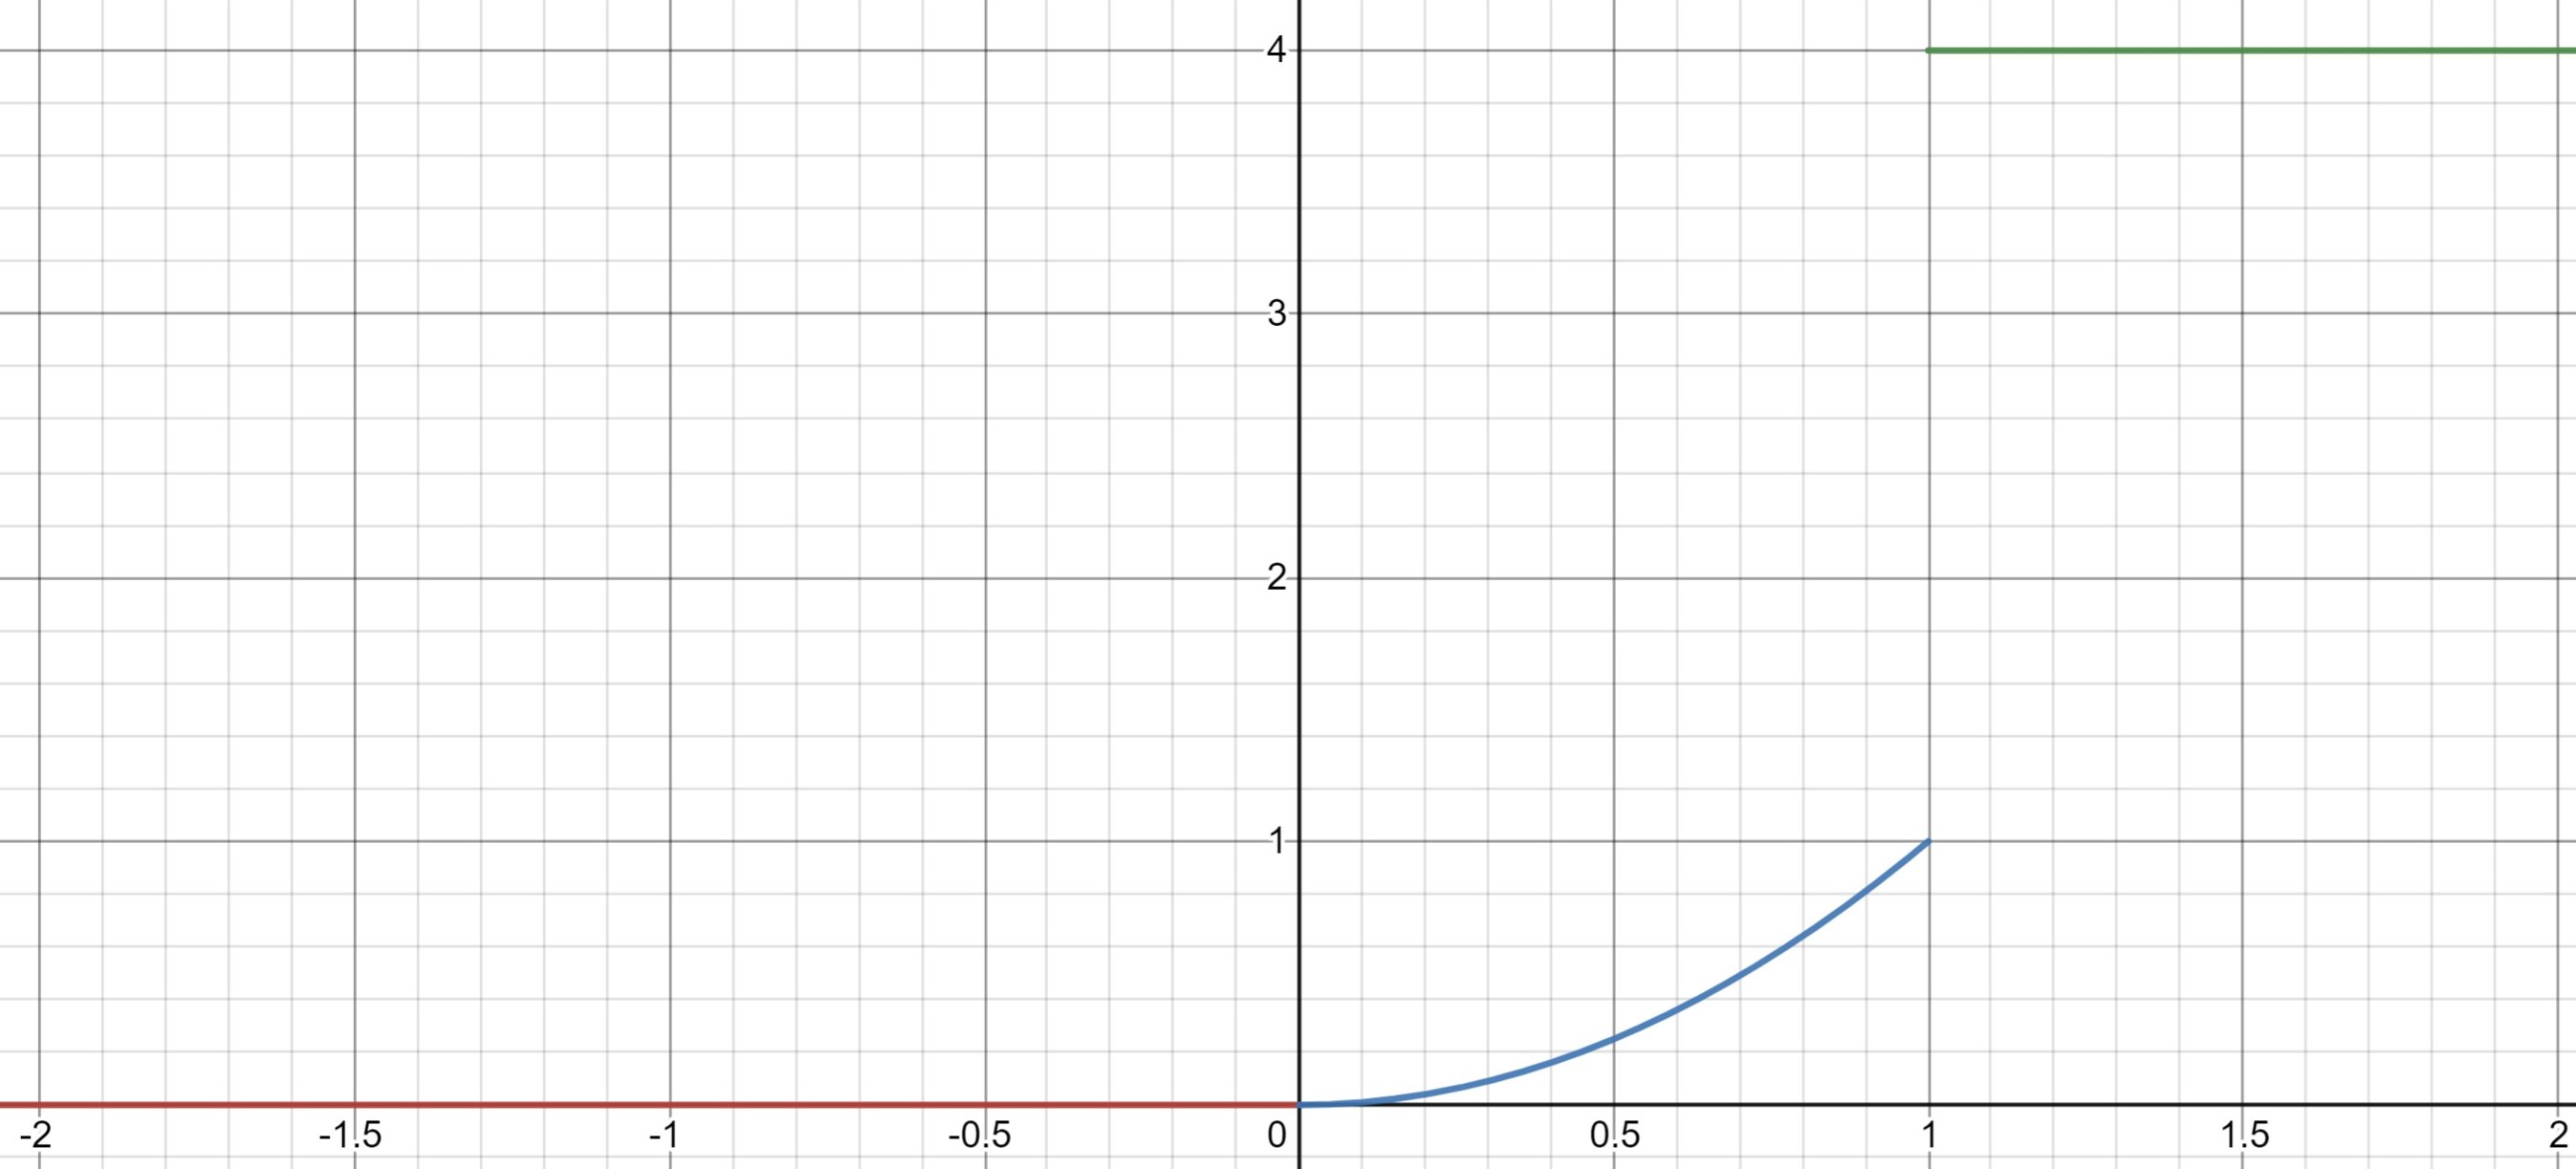
\includegraphics[scale=0.5]{graph F.JPG}\\
\end{center}
\vspace{\stretch{.5}}
$F$ is continuous on $\{x|x\neq1\}$\\
c. Where is $F$ differentiable and find $F'$ at those values.\\
$F$ is differentiable on $\{x|x\neq1\}$ and $F'=0$ for $x<0$, $F'=t$ for $0\leq x<1$, and $F'=4$ for $x>1$.\\[20pt]

6. Let $f$ be a continuous function on $\mathbb{R}$ and define $G(x)=\int_0^{\sin x}f(t)dt$ for $x\in\mathbb{R}$. Show $G$ is differentiable on $\mathbb{R}$ and compute $G'$.\\
Well, since $f$ is contionuous, $f$ is integrable. Now, since $f$ is continuous on $\mathbb{R}$ and $\sin x$ is continuous on $\mathbb{R}$, $f$ is continuous at $\sin x$ for all $x\in\mathbb{R}$. So by theorem 34.4, $G$ is differentiable and $G'(x)=f(\sin x)$.\\[20pt]

8.a,b. Use integration by parts to evaluate $\int_0^1x\arctan xdx$.\\
Let $u(x)=\arctan(x)$ and $v(x)=\frac{x^2+1}{2}$. Then $u'(x)=\frac{1}{1+x^2}$ and $v'(x)=x$. So, using intergration by parts, we get $$\int_0^1x\arctan xdx=(\arctan(x)\frac{x^2+1}{2})|_0^1-\int_0^1\frac{x^2+1}{2})(\frac{1}{1+x^2})dx=$$ $$(\arctan(x)\frac{x^2+1}{2})|_0^1-\int_0^1\frac12dx=$$ $$\frac{\pi}{4}-\frac12$$.\\[20pt]

9. Show $\int_0^{\frac12}\arcsin xdx=\frac{\pi}{12}+\frac{\sqrt{3}}{2}-1$.\\
Well, by example 3, we have that $\int_0^{\frac{\pi}{6}}\sin xdx+\int_0^{\frac12}\arcsin xdx=\frac12\frac{\pi}{6}=\frac{\pi}{12}$. Now, $\int_0^{\frac{\pi}{6}}\sin xdx=1-\frac{\sqrt{3}}{2}$. Therefore $1-\frac{\sqrt{3}}{2}+\int_0^{\frac12}\arcsin xdx=\frac12\frac{\pi}{6}=\frac{\pi}{12}$, and thus $\int_0^{\frac12}\arcsin xdx=\frac{\pi}{12}+\frac{\sqrt{3}}{2}-1$.\\[20pt]

\noindent Section 36\\

1. Show that if $f$ is integrable on $[a,b]$ then $\lim_{d\rightarrow b^-}\int_a^df(x)dx=\int_a^bf(x)dx$.\\
Well, since $f$ is integrable on $[a,b]$, $f$ is bounded on $[a,b]$. So, there exists some $M\in\mathbb{R}$ such that $M>0$ and $|f|\leq M$. So, $|\int_a^df(x)dx-\int_a^bf(x)dx|\leq M(b-d)$. Hence $\lim_{d\rightarrow b^-}|\int_a^df(x)dx-\int_a^bf(x)dx|=|\lim_{d\rightarrow b^-}\int_a^df(x)dx-\int_a^bf(x)dx|\leq \lim_{d\rightarrow b^-}M(b-d)=0$. Therefore $\lim_{d\rightarrow b^-}\int_a^df(x)dx=\int_a^bf(x)dx$ as desired.\\[20pt]

4.a. Calculate $\int_0^1\ln xdx$.\\
Well, $\int_0^1\ln xdx=\lim_{a\rightarrow0}\int_a^1\ln xdx=\lim_{a\rightarrow0}x\ln x-x|_a^1=1\ln1-1-\lim_{a\rightarrow0^+}a\ln a-a=-1-0=-1$.\\[20pt]

6. Let $f$ and $g$ be continuous functions on $(a,b)$ such that $0\leq f(x)\leq g(x)$ for all $x\in(a,b)$.\\
a. If $\int_a^bg(x)dx<\infty$ then $\int_a^bf(x)dx<\infty$.\\
Well, since $\int_a^bg(x)dx<\infty$, then $\int_a^bg(x)dx=M<\infty$. Thus $\int_a^bf(x)dx<\int_a^bg(x)dx=M$ and so $\int_a^bf(x)dx<\infty$ as desired.\\
b. If $\int_a^bf(x)dx=+\infty$, then $\int_a^bg(x)dx=+\infty$.\\
Well, by contrapositive, we have that if $\int_a^bg(x)dx<\infty$ then $\int_a^bf(x)dx<\infty$ which is proved above.\\[20pt]

7.a. Use 6 above to show $\int_{-\infty}^{\infty}e^{-x^2}dx<\infty$.\\
Well, for $x\geq1$, we have that $e^{-x^2}\leq e^{-x}$. Thus, $\int_{1}^{\infty}e^{-x^2}dx\leq\int_{1}^{\infty}e^{-x}dx=\frac1e$. So, by 6 above, we see that $\int_{-\infty}^{\infty}e^{-x^2}dx<\infty$.\\
b. Show this intergral equals $\sqrt{\pi}$.
Well,$(\int_{-\infty}^{\infty}e^{-x^2}dx)^2=\int_{-\infty}^{\infty}\int_{-\infty}^{\infty}e^{-x^2}e^{-y^2}dxdy=\int_{0}^{\infty}\int_{0}^{2\pi}e^{-r^2}rd\theta dr=2\pi\int_{0}^{\infty}e^{-r^2}rdr=2\pi\frac12(1-0)=\pi$ by u-substitution. Therefore $\int_{-\infty}^{\infty}e^{-x^2}dx=\sqrt{\pi}$.\\[20pt]

15.a. Give an examlpe of a sequence $(f_n)$ of integrable functions on $\mathbb{R}$ where $\int_{-\infty}^{\infty}f_n(x)dx=1$ for all $n$ and yet $f_n\rightarrow0$ uniformly on $\mathbb{R}$.\\
Well, $f_n(x)=\frac{1}{n+1}$ for $x\in[0,n+1]$ and $f_n(x)=0$ elsewhere. So, $\int_{-\infty}^{\infty}f_n(x)dx=\int_{-\infty}^{0}0dx+\int_{0}^{n+1}\frac{1}{n+1}dx+\int_{n+1}^{\infty}0dx=0+1+0=1$. However, $f_n\rightarrow0$ uniformly on $\mathbb{R}$.





\end{document}